\documentclass{ctexart}
\usepackage{graphicx}



\title{信息内容安全实验技术报告 }
\author{\\\\项目名称:微博的内容识别与控制\\\\ 韦昆杰  \\\\ 1181000420 \\\\  348971397@qq.com  \\\\\\\\\\\\\\\\\\\\\\\\\\\\}
\date{\today}

\graphicspath{{images/}}
\begin{document}
\maketitle
\newpage
\tableofcontents

\section{摘要}
本实验主要实现了一个小型的信息安全管理系统,其中包含以下功能:
\subsection{网络信息数据分类捕获}
\begin{enumerate}
    \item 通过爬虫对微博进行爬取,得到HTML
    \item 通过对HTML的进一步提取分析,得到信息
\end{enumerate}

\subsection{网络协议还原分析}
\begin{enumerate}
    \item 实现了常见的字符串匹配算法(BF KMP AC)
    \item 当关键字为一个时采用KMP算法匹配,当关键字为多个时采用AC算法匹配
    \item 通过将获取的信息进行关键字匹配,可以识别包含指定关键字的页面
\end{enumerate}
\subsection{网络信息内容或报文特征识别}
\begin{enumerate}
    \item 采用主流的字符串匹配算法,匹配其中的主题相关关键词。
    \item 还可以进行离线的分析,得到主题的统计结果
\end{enumerate}

\subsection{网络信息安全管理响应}
\begin{enumerate}
    \item 针对前面匹配到的关键字或者网站地址,设计并实现有效的控管操作
    \item 采用水军的引导方法,使得某微博被淹没
    \item 通过举报匹配到的微博使其被删除
\end{enumerate}

\subsection{系统辅助功能部分}
\begin{enumerate}
    \item MongoDB数据库存储爬取的热搜榜以及微博信息
    \item 实现了网站页面,用户可以通过GUI完成各项操作
\end{enumerate}

本系统在Windows10平台上进行开发和测试,使用的开发环境为Visual Studio Code,开发语言为TypeScript,使用的数据库为MongoDB数据库,网站页面使用HTML CSS实现,网站爬取采用puppeteer实现。
\section{项目简介}


\subsection{背景分析}
了解信息安全管理系统设计的关键环节,掌握网络信息内容的高效的数据捕获技术、准确识别及分析各种常用协议报文,并可针对用户的屏蔽内容需要,拦截或统计分析相应的特征报文。能够针对信息内容安全领域的新进展、新应用,设计与开发实用化的网络信息监控系统。
\subsection{特色描述}
通过主动爬虫爬取微博,得到微博信息,存储到数据库中。然后设置关键字,通过匹配算法进行匹配,并对匹配到的微博进行管控(水军或举报)

\section{实现方案}

\subsection{系统方案}

系统平台: Windows 10

开发语言: TypeScript

界面实现: HTML CSS

数据库系统: MongoDB数据库

\subsection{实现原理}

\subsubsection{微博热搜子系统}
实时爬取微博当前的热搜,并在网页端展示出来,并存储到数据库中
\subsubsection{微博搜索子系统}
输入要搜索的内容,系统爬取相关微博展示,爬取到的所有微博信息存储到数据库中
\subsubsection{微博过滤子系统}
设置关键字,系统采用KMP或AC算法对微博进行匹配,匹配到的微博展示到网页上
\subsubsection{微博管控子系统}
对匹配到的微博,可以进行管控,通过举报该微博或进行相关信息微博的不断发生淹没该微博
\subsubsection{数据库子系统}
这里借助MongoDB数据库,设计数据库操作子系统,将微博信息存储到数据库中
\subsubsection{图形化界面子系统}
利用HTML CSS设计网页UI,TypeScript实现动态交互
\subsection{硬件框图}
本系统不涉及硬件结构
\subsection{系统软件流程}
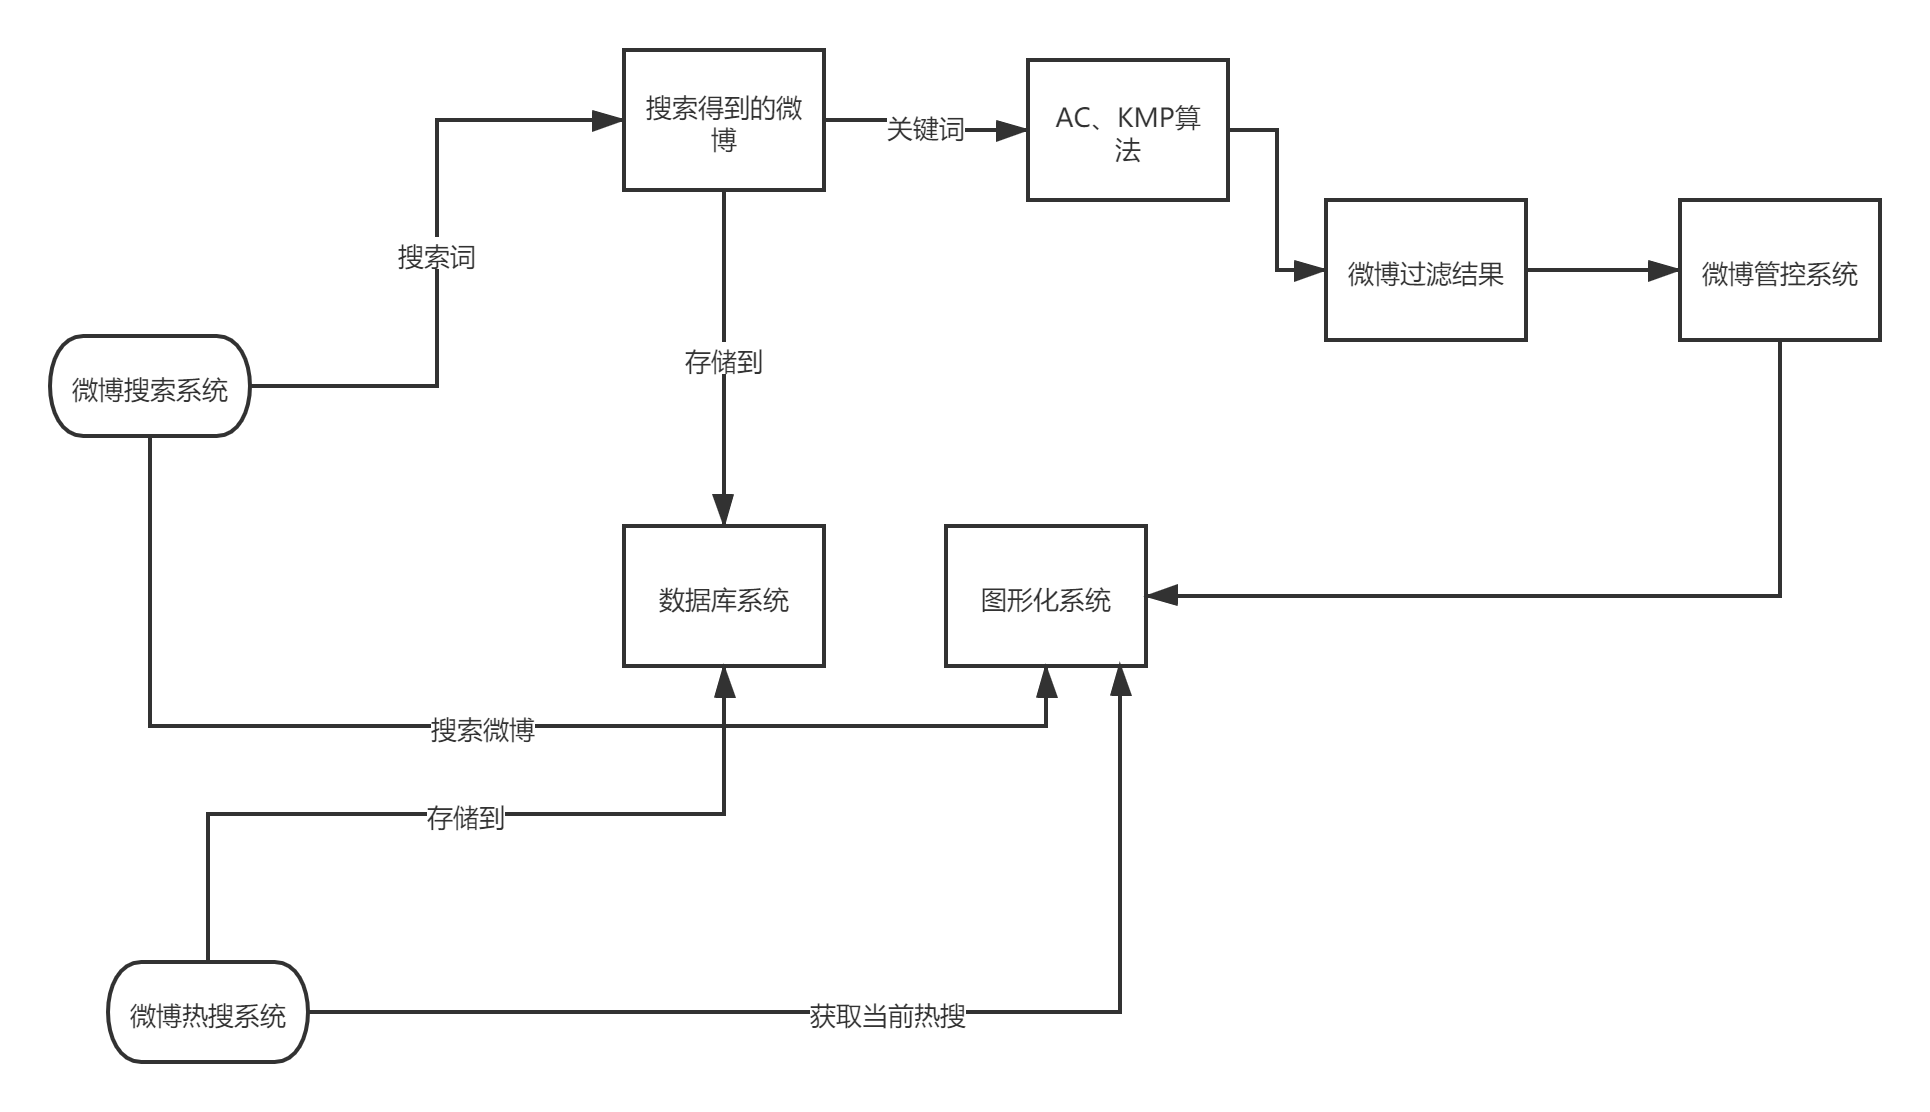
\includegraphics[width=\textwidth]{chart.png}
\section{系统功能设计}

\subsection{微博热搜子系统}
该系统通过HTTP请求热搜网页,得到对应的HTML后对其进行进一步的提取分析,得到微博热搜编号、内容、搜索量
信息,将这些信息存储到数据库中并且展示在页面上
\subsection{微博搜索子系统}
该系统接受用户搜索,通过HTTP命令得到搜索对应的微博HTML,解析HTML得到各条微博的URL,
通过Puppeteer模拟分别爬取各条微博的内容。得到微博URL、发送用户、微博发送时间、微博内容、
点赞数、评论数、转发数等信息存储到数据库中,并展示在页面上
\subsection{微博过滤子系统}
该系统接受用户输入关键词,系统根据关键词个数(如果为1采用KMP算法,否则采用AC算法)进行匹配,匹配后的结果展示在页面上
\subsection{微博管控子系统}
用户可以选择是否对过滤到的微博进行管控,如果选择管控,系统会通过Puppeteer(需要一个登录的账号,模拟真实的微博用户)对相应微博进行举报或者产生大量相同内容微博
\subsection{数据库子系统}
数据库采用MongoDB,对收集到的热搜信息和微博信息分别存储到相应的Collection中,可以随时查看
\subsection{图形化界面子系统}
本实验采用网页,通过HTML CSS设计网页UI,TypeScript实现动态交互

\section{关键技术}
\subsection{KMP算法}
当关键词个数为1时,微博过滤子系统采用KMP算法对微博内容进行匹配。

KMP算法首先通过计算模式串的最长公共前后缀,并将结果存储到表中,并根据该表进行匹配。
一个词在不匹配时本身就包含足够的信息来确定下一个匹配可能的开始位置,此算法利用这一特性以避免重新检查先前匹配的字符。

该算法时间复杂度为O(m)+O(n),空间复杂度为O(m)
\subsection{AC算法}
当关键词个数超过1个时,微博过滤系统采用AC算法对微博内容进行匹配。

AC算法在初始阶段,建立三个函数,转向函数goto,失效函数故障和输出函数输出,
在搜索查找中,通过这三个函数的交叉使用扫描,定位出关键字在文本中的所有
出现位置

该软件扫描文本时完全无需回溯,时间复杂度为O(n),时间复杂度与关键字的数量和长度无关系
\subsection{React}
React(有时叫 React.js 或 ReactJS),是一个为数据提供渲染为 HTML 视图的开源 JavaScript 库。React 视图通常采用包含以自定义 HTML 标记规定的其他组件的组件渲染。React 为程序员提供了一种子组件不能直接影响外层组件(data flows down)的模型,数据改变时对 HTML 文档的有效更新,和现代单页应用中组件之间干净的分离。

本实验采用React,通过JSX(JavaScript XML)描述页面结构,最终渲染为HTML
\subsection{Puppeteer}
Puppeteer 是一个 Node 库,它提供了一个高级 API 来通过 DevTools 协议控制 Chromium 或 Chrome。

本实验采用Puppeteer,模拟微博用户实现微博爬取和微博举报等功能
\section{总结}
本实验主要实现了一个小型的信息安全管理系统,实现了对动态网页(微博网页版)的内容识别与控制

\section{参考文献}
\begin{itemize}
    \item KMP算法-维基百科 [https://zh.wikipedia.org/wiki/KMP算法]
    \item AC算法-维基百科 [https://zh.wikipedia.org/wiki/AC自动机算法]
    \item React-维基百科 [https://zh.wikipedia.org/wiki/React]
    \item Puppeteer [https://pptr.dev/]
\end{itemize}
\end{document}
